\begin{figure}[ht]
 \centering
 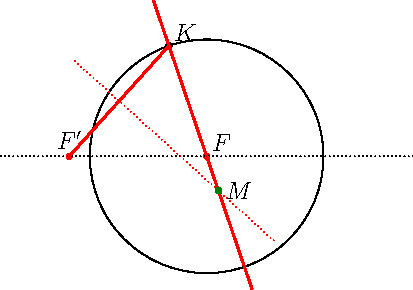
\includegraphics[width=5cm]{Eco06_1.pdf}
 % Eco06_1.pdf: 198x139 px, 72dpi, 6.99x4.90 cm, bb=0 0 198 139
 \caption{Exercice \arabic{enumi} : cas $a<c$}
 \label{fig:Eco6_1}
\end{figure}
\begin{figure}[ht]
 \centering
 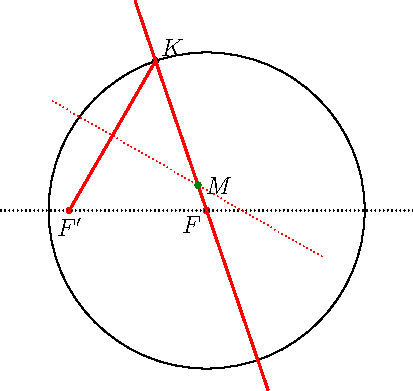
\includegraphics[width=5cm]{Eco06_2.pdf}
 % Eco06_1.pdf: 198x139 px, 72dpi, 6.99x4.90 cm, bb=0 0 198 139
 \caption{Exercice \arabic{enumi} : cas $a>c$}
 \label{fig:Eco6_2}
\end{figure}

\begin{tiny}(Eco06)\end{tiny} Cercle directeur.\newline
Soit $c>0$ et deux points $F$ et $F'$ avec $FF'=2c$, le cercle $\mathcal C$ est centré en $F$ et de rayon $2a$ ($a>0$).\newline
\`A tout point $K$ de $\mathcal C$, on associe le point d'intersection $M$ (lorsqu'il existe) de la médiatrice de $[F',K]$ avec la droite $(KF)$. On devra considérer les deux cas (figure \ref{fig:Eco6_1} et figure \ref{fig:Eco6_2}).
\begin{enumerate}
 \item Préciser le cas dans lequel la médiatrice de $[F',K]$ et la droite $(KF)$ ne se coupent pas.
 \item Montrer que lorsque $K$ décrit $\mathcal C$, le point $M$ décrit une conique à préciser. On dit que $\mathcal C$ est le \emph{cercle directeur} de la conique.
 \item On paramètre le cercle directeur par 
\begin{displaymath}
 \theta \rightarrow K(\theta) = F +2a\overrightarrow{e_\theta}
\end{displaymath}
et on note $M(\theta)$ le point correspondant. Calculer $M(\theta)$ et $\overrightarrow {M'} (\theta)$. En déduire que la médiatrice de $[F'K]$ est la tangente en $M$ à la conique.
\item Quelle est la courbe formée par les projetés orthogonaux de $F'$ sur les tangentes à la conique (podaire) ? \index{podaire}
\end{enumerate}
